%% 
%% Copyright 2007-2024 Elsevier Ltd
%% 
%% This file is part of the 'Elsarticle Bundle'.
%% ---------------------------------------------
%% 
%% It may be distributed under the conditions of the LaTeX Project Public
%% License, either version 1.3 of this license or (at your option) any
%% later version.  The latest version of this license is in
%%    http://www.latex-project.org/lppl.txt
%% and version 1.3 or later is part of all distributions of LaTeX
%% version 1999/12/01 or later.
%% 
%% The list of all files belonging to the 'Elsarticle Bundle' is
%% given in the file `manifest.txt'.
%% 
%% Template article for Elsevier's document class `elsarticle'
%% with numbered style bibliographic references
%% SP 2008/03/01
%% $Id: elsarticle-template-num.tex 249 2024-04-06 10:51:24Z rishi $
%%
% \documentclass[preprint,12pt]{elsarticle}

%% Use the option review to obtain double line spacing
\documentclass[authoryear,preprint,review,12pt]{elsarticle}

%% Use the options 1p,twocolumn; 3p; 3p,twocolumn; 5p; or 5p,twocolumn
%% for a journal layout:
%% \documentclass[final,1p,times]{elsarticle}
%% \documentclass[final,1p,times,twocolumn]{elsarticle}
%% \documentclass[final,3p,times]{elsarticle}
% \documentclass[final,3p,times,twocolumn]{elsarticle}
% \documentclass[final,5p,times]{elsarticle}
% \documentclass[final,5p,times,twocolumn]{elsarticle}

%% For including figures, graphicx.sty has been loaded in
%% elsarticle.cls. If you prefer to use the old commands
%% please give \usepackage{epsfig}

%% The amssymb package provides various useful mathematical symbols
\usepackage{amssymb}
%% The amsmath package provides various useful equation environments.
\usepackage{amsmath}
\usepackage{pifont}
%% The amsthm package provides extended theorem environments
%% \usepackage{amsthm}

%% USER-DEFINED SHORTCUTS
\usepackage{siunitx}
\usepackage{caption}
\usepackage{subcaption}
\usepackage[dvipsnames]{xcolor}
\usepackage{comment}
\newcommand{\mrm}[1]{\mathrm{#1}}
\newcommand{\taup}{\tau_\mathrm{p}}   
\newcommand{\taui}{\tau_\mathrm{i}}   
\newcommand{\taub}{\tau_\mathrm{b}}   
\newcommand{\tauc}{\tau_\mathrm{c}}   
\newcommand{\taue}{\tau_\mathrm{e}}  
\newcommand{\tauk}{\tau_\mathrm{\eta}}   
\newcommand{\tauL}{\tau_L} 

% \newcommand{\red}{\color{red}}
% \newcommand{\blue}{\color{blue}}
% \newcommand{\green}{\color{ForestGreen}}
% \newcommand{\orange}{\color{orange}}
% \newcommand{\pink}{\color{Salmon}}

\newcommand{\red}{}
\newcommand{\blue}{}
\newcommand{\green}{}
\newcommand{\orange}{}
\newcommand{\pink}{}

%% \begin{linenumbers}, end it with \end{linenumbers}. Or switch it on
%% for the whole article with \linenumbers.
%% \usepackage{lineno}


\journal{Fuel}

\begin{document}

\begin{frontmatter}

%% Title, authors and addresses

%% use the tnoteref command within \title for footnotes;
%% use the tnotetext command for theassociated footnote;
%% use the fnref command within \author or \affiliation for footnotes;
%% use the fntext command for theassociated footnote;
%% use the corref command within \author for corresponding author footnotes;
%% use the cortext command for theassociated footnote;
%% use the ead command for the email address,
%% and the form \ead[url] for the home page:
%% \title{Title\tnoteref{label1}}
%% \tnotetext[label1]{}
%% \author{Name\corref{cor1}\fnref{label2}}
%% \ead{email address}
%% \ead[url]{home page}
%% \fntext[label2]{}
%% \cortext[cor1]{}
%% \affiliation{organization={},
%%             addressline={},
%%             city={},
%%             postcode={},
%%             state={},
%%             country={}}
%% \fntext[label3]{}

\title{A Theoretical Analysis of Timescales in Preferential Concentration of Burning Iron Particles}

%% use optional labels to link authors explicitly to addresses:
%% \author[label1,label2]{}
%% \affiliation[label1]{organization={},
%%             addressline={},
%%             city={},
%%             postcode={},
%%             state={},
%%             country={}}
%%
%% \affiliation[label2]{organization={},
%%             addressline={},
%%             city={},
%%             postcode={},
%%             state={},
%%             country={}}

\author[label1,label2]{Shyam Hemamalini} %% Author name
\author[label1]{Benedicte Cuenot}
\author[label1,label2]{XiaoCheng Mi}

%% Author affiliation
\affiliation[label1]{
            organization={Department of Mechanical Engineering, Eindhoven University of Technology},%Department and Organization
            addressline={Groene Loper 3}, 
            city={Eindhoven},
            postcode={5600MB}, 
            country={The Netherlands}}

\affiliation[label2]{
            organization={Eindhoven Institute for Renewable Energy Systems},%Department and Organization
            addressline={Groene Loper 3}, 
            city={Eindhoven},
            postcode={5600MB}, 
            country={The Netherlands}}
%% Abstract
\begin{abstract}
%% Text of abstract
Preferential concentration in iron powder combustion is highly probable owing to the particle-laden turbulent flow. \iffalse However, under which conditions does clustering impact the preheating and the combustion process?  To answer this,\fi A theoretical analysis on the timescales relevant to the combustion process and the dynamics of preferential concentration -- particle relaxation timescale $\taup$, preheating timescale $\taui$, combustion timescale $\taub$, cluster formation timescale $\tauc$ and cluster evolution timescale $\taue$ -- is presented in this work assuming homogeneous isotropic turbulence. Comparison of the timescales with $\taup$ as reference results in simplified ratios with thermophysical constants and few independent parameters. Under parameter ranges of gas-phase $\mathrm{O_2}$ mass fraction $Y_\mrm{O_2}$ and bulk Reynolds number $\mrm{Re}_L$  commonly seen in large scale turbulent iron powder burners, it is estimated that $\taui <\tauc$ thus, particle preheating is likely faster than the cluster formation. \iffalse At air-like conditions, $\taub < \tauc$ and hence, most ignited particles are expected to fully burn out before the clusters have been formed. However, $\taub \approx \tauc$ at lower $Y_\mrm{O_2}<0.05$, and in such conditions, the dynamics of cluster formation might influence the combustion process. An analysis of $\taub/\taue$ is presented based on the values of $\mrm{St}$, $\mrm{Re}_L$ and $Y_\mrm{O_2}$ from which the interaction of the combustion process with the cluster dynamics can be predicted. Under realistic conditions, $\taub \ll \taue$ such that the cluster evolution dynamics are not expected to interact with the combustion process, and can be neglected.\fi Different scenarios based on $\taub/\tauc$ and $\taub/\taue$ are hypothesized: If $\taub < \tauc$, combustion is complete before the formation of clusters and hence, only the initial particle distribution is relevant; if $\taub\gtrsim\tauc$ and $\taub < \taue$, combustion occurs completely in a clustered particle distribution and the effects of preferential concentration are maximised; if $\taub > \taue$, the particles move freely in and out of clusters that the effects of preferential concentration on the oxidation are reduced. This simplified analysis, though not directly relatable to real-world applications, is intended to highlight (or eliminate) parameter ranges at which preferential concentration can have an increased (or negligible) effect on combustion. 
\end{abstract}
% \begin{comment}
%%Graphical abstract
\begin{graphicalabstract}
\begin{figure}[h]
     \centering
     \includegraphics[width=0.88\linewidth]{plots/graphicalabstract3.pdf}
% \caption{Caption}
     \label{fig:scenarios}
\end{figure}
 \end{graphicalabstract}

% %%Research highlights
\begin{highlights}
% \iffalse
% \item The relevant timescales for the preferential concentration of iron particles in turbulent iron powder combustion are categorized as particle relaxation timescale $\taup$, preheating timescale $\taui$, combustion timescale $\taub$, cluster formation timescale $\tauc$ and cluster evolution timescale $\taue$, in addition to the Kolmogorov timescale $\tauk$ and integral timescale $\tauL$.\fi
 \item A theoretical analysis of the timescales involved in the preferential concentration of iron particles in turbulent iron powder combustion shows that, 
 \begin{itemize}
     \item preheating timescale $\taui$ is much smaller than the cluster formation timescale $\tauc$ across a wide range of conditions, and hence, preheating is likely not affected by clustering.
%     \iffalse \item combustion timescale $\taub$ is smaller than the cluster formation timescale $\tauc$ at air-like conditions, however, $\taub/\tauc$ approaches unity at lower $Y_\mrm{O_2}$. Ignited particles likely burn out before cluster stabilization, however, there could be two-way effects of cluster formation and combustion processes at lower $Y_\mrm{O_2}$.\fi
     \item  $\taub/\tauc$ and $\taub/\taue$ based on $Y_\mrm{O_2}$, $\mrm{Re}_L$ and $\mrm{St}_\eta$ may be essential in estimating the effect of cluster dynamics on the combustion process.
     \item if $\taub < \tauc$, the particles combust completely before stabilizing into clusters, no effects of preferential concentration are seen in the combustion process, only the initial distribution is relevant; if $\taub \gtrsim \tauc$ and $\taub < \taue$, interaction between the processes might be significant and the effects of preferential concentration on the combustion process may be maximised; if $\taub \gtrsim \taue$, particles move freely through clusters and hence, the effect of clustering on the combustion process might be negligible.
%     \iffalse \item combustion timescale $\taub$ is much smaller than the cluster evolution timescale $\taue$ at $\mrm{Re}_L > 1000$, and hence, the combustion process is unaffected by cluster evolution, and the particle distribution might be ``frozen" from the perspective of the combustion.\fi
 \end{itemize}
 \item The simplified analysis is intended to highlight or eliminate parameter ranges at which preferential concentration might be significant or insignificant to the combustion process.
 \end{highlights}
% \end{comment}
%% Keywords
\begin{keyword}
%% keywords here, in the form: keyword \sep keyword
Iron powder combustion \sep Preferential concentration \sep Turbulence
%% PACS codes here, in the form: \PACS code \sep code

%% MSC codes here, in the form: \MSC code \sep code
%% or \MSC[2008] code \sep code (2000 is the default)

\end{keyword}

\end{frontmatter}

%% Add \usepackage{lineno} before \begin{document} and uncomment 
%% following line to enable line numbers
%% \linenumbers

%% main text
%%

\section{Introduction}\label{sec:introduction}

\iffalse
{Understanding of the two-way interaction of turbulence with burning iron particles is nascent \cite{Hemamalini2024, Luu2024}, albeit highly significant from the perspective of large-scale design.}
\fi
{\green
Iron powders (i.e., \SI{10}{\micro\meter} to \SI{100}{\micro\meter}-sized particles) are a novel, renewable, and cyclic energy carrier that has seen rapid development in research and design over the past decade. At the time of writing, large-scale iron-powder combustors are operational, delivering power outputs in the range of hundreds of kilowatts~\cite{niekthesis}. In these pilot-scale combustors, iron particles burn under turbulent flow conditions.

Since the combustion temperature of iron particles in air is lower than the boiling points of liquid iron and iron oxide, the combustion process is primarily heterogeneous and non-volatile, involving minimal evaporation. This behavior contrasts with that of volatile metal fuels (e.g., aluminium, magnesium) and many pulverized hydrocarbon-based solid fuels (e.g., biomass and coal), which undergo devolatilization followed by gas-phase oxidation. Therefore, in the aforementioned large-scale combustors, condensed-phase iron particles interact with turbulence throughout their combustion. In such particle-laden turbulent flows, a phenomenon known as \textit{preferential concentration} arises due to a resonance between particle and flow relaxation times. This leads to the formation of particle-rich regions (clusters) and particle-sparse regions (voids). Recently, experimental evidence of particle clustering has also been observed in a lab-scale iron-powder burner~\cite{STEFFENS2025}.

Preferential concentration in non-reacting particle-laden turbulent flows has been widely studied. The first theoretical framework was introduced by Eaton and Fessler~\cite{Eaton1994}, with subsequent contributions from the fluid dynamics community significantly advancing the understanding of this phenomenon. Monchaux et al. \cite{Monchaux2012} offer a detailed overview of experimental and numerical research on preferential concentration and methods to quantify it. Recent parametric studies by Sumbekova et al. \cite{Sumbekova} and Uhlmann and Chouippe~\cite{Uhlmann} have investigated its behavior across a wide range of Stokes numbers, turbulent Reynolds numbers, and particle loadings. These studies primarily focus on sub-Kolmogorov particles, although similar research on larger particles has also been conducted.

The impact of preferential concentration on turbulent iron-powder combustion remains underexplored. Due to challenges in obtaining in-situ data from industrial-scale systems, researchers have proposed various alternative configurations to study this process computationally, such as mixing layers with decaying turbulence~\cite{Hemamalini2024,Luu2024}, forced homogeneous isotropic turbulence (HIT)~\cite{Thaeter2024}, and conical jets in miniaturized swirl combustors~\cite{STEFFENS2025}. In these prior numerical studies~\cite{Hemamalini2024,Luu2024,Thaeter2024}, the flow conditions are tailored to induce preferential concentration that influences iron particle combustion. However, a more general question remains: under what conditions is preferential concentration coupled with iron-particle combustion?

Unlike previous studies focused on specific flow setups, this brief communication presents a simplified analysis to develop a broader understanding of the key timescales involved in turbulent iron-powder combustion. The relevant particle timescales are the relaxation timescale $\tau_\mathrm{p}$, preheating timescale before ignition $\tau_\mathrm{i}$, and combustion timescale $\tau_\mathrm{b}$. Flow timescales include the integral timescale $\tau_L$ and Kolmogorov timescale $\tauk$. Clustering timescales are cluster formation timescale $\tau_\mathrm{c}$ and evolution timescale $\tau_\mathrm{e}$. By estimating and comparing these timescales, this analysis aims to provide a general framework to assess the extent of coupling or decoupling between combustion and preferential concentration driven by particle–turbulence interactions.} {\red Phenomena such as interparticle collisions and polydispersity in the particle distribution have been excluded from this study. Their influence on combustion and turbulence is complex and dynamic, and addressing them would require detailed and computationally intensive simulations, which are beyond the scope of this work.}

\section{Description of the timescales}\label{sec:description}

Three timescales characterizing the flow interaction and combustion process of an iron particle are defined -- \textit{relaxation timescale} $\tau_\mathrm{p}$, \textit{preheating timescale} $\tau_\mathrm{i}$ and \textit{combustion timescale} $\tau_\mathrm{b}$. $\taup$ is defined from the Stokes drag force as
\begin{equation}
    \taup = \frac{\rho_\mrm{p} d_\mrm{p}^2}{18 \mu_\mrm{g}} \label{eq:taup}
\end{equation}
\noindent where $\rho_\mrm{p} = \rho_\mrm{Fe}$ is the particle density, $d_\mrm{p}$ the particle diameter, $\rho_\mrm{g}$ and $\nu_\mrm{g}$ the density and the kinematic viscosity of the gas respectively. {\red At higher particle Reynolds numbers, a drag correction term $C_\mrm{d}$ is often incorporated into the particle relaxation timescale. However, this term is not expected to change the order of magnitude of $\taup$ in the scales of interest for small particle Reynolds numbers, and is hence not considered in this analysis for the sake of simplicity.}

The \textit{preheating timescale} $\tau_\mrm{i}$ is approximated as the timescale for the particle initially at temperature $T_\mrm{p}$ to be heated to the single-particle ignition threshold temperature $T_\mrm{i}$. The heating rate pre-ignition is assumed to be driven by convective heat transfer from the gas to the particle rather than solid state kinetics. $\taui$ can be estimated as a linear approximation through the ratio of the energy $Q_{\mrm{p} \rightarrow \mrm{i}}$ required to raise the particle temperature from $T_\mrm{p}$ to $T_\mrm{i}$, and the heat transfer rate $\dot{Q}_{\mrm{g} \rightarrow \mrm{p}}$ from the gas at $T_\mrm{g}$ to the particle at $T_\mrm{p}$ as:
{\blue
\begin{equation}
    \taui =  \frac{Q_{\mrm{p} \rightarrow \mrm{i}}}{\dot{Q}_{\mrm{g} \rightarrow \mrm{p}}} \label{eq:taui0}
\end{equation}

\noindent$Q_{\mrm{p} \rightarrow \mrm{i}}$ and $\dot{Q}_{\mrm{g} \rightarrow \mrm{p}}$ can be expanded as:
\begin{eqnarray}
    Q_{\mrm{p} \rightarrow \mrm{i}} &=& \rho_\mathrm{Fe} \ V_\mathrm{p}\cdot c_\mathrm{p,Fe}(T_\mathrm{i} - T_\mathrm{p})\\
    \dot{Q}_{\mrm{g} \rightarrow \mrm{p}} &=& hA_\mathrm{p} \cdot |T_\mathrm{g} - T_\mathrm{p}|
\end{eqnarray}
\noindent where $c_\mrm{p,Fe}$ is the specific heat capacity of $\mrm{Fe}$, $V_\mrm{p}$ and $A_\mrm{p}$ the volume and surface area of the particle, and $h$ the convective heat transfer coefficient. Assuming a perfectly spherical particle with negligible slip velocity, i.e., $\mrm{Nu}=2$, Equation \ref{eq:taui0} can be expressed as:
\begin{equation}
    \taui = \frac{\rho_\mrm{Fe} c_\mrm{p,Fe} d_\mrm{p}^2}{12 k_\mrm{g}} \cdot \frac{T_\mrm{i} - T_\mrm{p}}{T_\mrm{g} - T_\mrm{p}} \label{eq:taui}
\end{equation}
where $k_\mrm{g}$ is the thermal conductivity of the gas.}

$\taui$ is dependent on $d_\mrm{p}$, $T_\mrm{p}$ and $T_\mrm{g}$, and Figure \ref{fig:taui} shows the estimation of $\tau_\mrm{i}$ for a range of $d_\mrm{p}$, $T_\mrm{g}$ and $T_\mrm{p}$, assuming $T_\mrm{i}=\SI{1082}{\kelvin}$ following the analysis on iron particle ignition by Mi et al. \cite{Mi2022}. Note that $\taui$ is  only weakly sensitive to $T_\mrm{p}$ and $T_\mrm{g}$ with values within the same order of magnitude for the range considered, whereas $d_\mrm{p}$ has a quadratic effect on $\taui$.

\begin{figure}
    \centering
    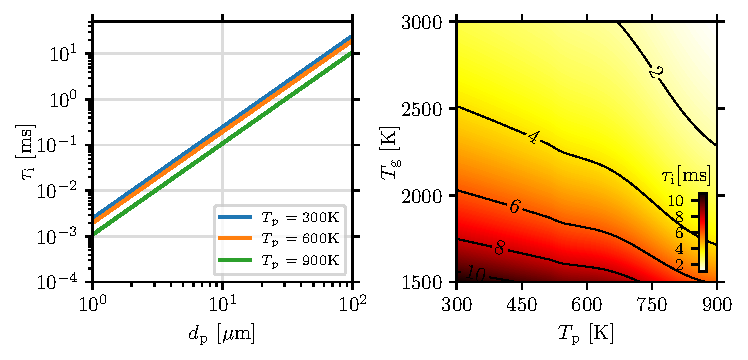
\includegraphics[width=0.9\linewidth]{plots/taui.pdf}
    % \vspace{-30pt}
    \caption{Estimation of preheating timescale $\taui$ from Equation \ref{eq:taui}. Left figure shows the variation in $\taui$ with particle size $d_\mrm{p}$ with $T_\mrm{g}=\SI{2000}{\kelvin}$ and $T_\mrm{i} = \SI{1082}{\kelvin}$ at different $T_\mrm{p} = [300, 600,900]\, \SI{}{\kelvin}$. Right figure shows the variation in $\taui$ with respect to initial particle temperature $T_\mrm{p}$ and gas temperature $T_\mrm{g}$ with $d_\mrm{p}=\SI{50}{\micro\meter}$. Gas properties are evaluated at $T_\mrm{g}$.}
    \label{fig:taui}
\end{figure}

The \textit{combustion timescale} $\taub$, is approximated as the time taken for the completion of oxidation of iron in the particle into its oxides. For simplicity, only the first oxidation state approximated by liquid FeO is considered, and the gaseous medium is assumed to consist of only $\mrm{O_2}$ and $\mrm{N_2}$. $\taub$ is then described as a linear approximation through the ratio of the mass of $\mrm{Fe}$ in the particle and the mass consumption rate of $\mrm{Fe}$ assuming external diffusion of $\mrm{O_2}$ from the bulk to the particle surface as the rate-limiting process. {\red Note that the oxidation through solid state kinetics has been ignored in this analysis for the estimation of $\taub$, as prior work \cite{Ning2021,ning2024experimental,Thijs2023,fujinawa2023,thijs2023surface} show that external oxygen transport is the dominant rate-limiting process at lower (realistic) $Y_\mrm{O_2}$.}
{\iffalse The assumption of oxygen diffusion across the boundary layer of the particle being the rate-limiting process for combustion is motivated by the works of Ning et al. \cite{ning2024experimental} and Kuhmann et al. \cite{kuhmann2025optimised}.\fi}
{\blue
\begin{equation}
    \taub = \frac{m_\mrm{p}}{\dot{m}_\mrm{Fe,D,max}} \label{eq:taub0}
\end{equation}
The mass consumption of $\mrm{Fe}$ based on oxygen diffusion $\dot{m}_\mrm{Fe,D}$ is given by
\begin{equation}
    \dot{m}_\mrm{Fe,D} = s_\mrm{FeO} A_\mrm{p} \beta_\mrm{p} (\rho_\mrm{O_2,g} - \rho_\mrm{O_2,s})
\end{equation}
where $s_\mrm{FeO}$ is the stoichiometric mass ratio between $\mrm{Fe}$ and $\mrm{O_2}$ for the single-stage oxidation to $\mrm{FeO}$, $\beta_\mrm{p} = \mrm{Sh}D_\mrm{O_2}/d_\mrm{p}$ the mass transfer coefficient with $D_\mrm{O_2}$ the mass diffusivity of $\mrm{O_2}$, $\rho_\mrm{O_2,g}$ and $\rho_\mrm{O_2,s}$ represent the concentration of oxygen in the bulk gas and at the particle surface, respectively. When oxygen diffusion is the rate-limiting process, the concentration of oxygen at the particle surface is zero ($\rho_\mrm{O_2,s} = 0$), and the mass consumption of $\mrm{Fe}$ assuming oxygen diffusion is maximum, and is given by $\dot{m}_\mrm{Fe,D,max}$. $m_\mrm{p}$ and $\dot{m}_\mrm{Fe,D,max}$ can be expanded as:
\begin{eqnarray}
   m_\mrm{p} &=& \rho_\mrm{Fe} V_\mrm{p} \\
    \dot{m}_\mrm{Fe,D,max} &=& s_\mrm{FeO} A_\mrm{p} \beta_\mrm{p} \rho_\mrm{O_2}
\end{eqnarray}
Consistently assuming a perfectly spherical particle with negligible slip velocity, i.e., $\mrm{Sh}=2$, we have:
\begin{equation}
    \taub = \frac{\rho_\mrm{Fe} d_\mrm{p}^2}{12 s_\mrm{FeO} D_\mrm{O_2} \rho_\mrm{g} Y_\mrm{O_2}} \label{eq:taub}
\end{equation}
 where $Y_\mrm{O_2}$ the mass fraction of $\mrm{O_2}$ in the gas phase. Figure \ref{fig:taub} shows the estimation of $\taub$ with respect to $d_\mrm{p}$ and $T_\mrm{g}$ and $Y_\mrm{O_2}$. Since $D_\mrm{O_2}$ also depends on $T_\mrm{g}$, the variation of $\taub$ with respect to $T_\mrm{g}$ is considered. However, Figure \ref{fig:taub} shows only a weak dependence on $T_\mrm{g}$, an inverse linear relationship with $Y_\mrm{O_2}$ and a quadratic dependence on $d_\mrm{p}$.
}
\begin{figure}
    \centering
    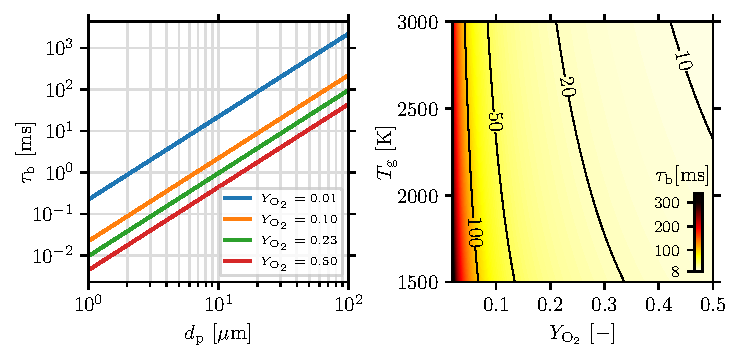
\includegraphics[width=0.9\linewidth]{plots/taub.pdf}
    % \vspace{-30pt}
    \caption{Estimation of combustion timescale $\taub$ from Equation \ref{eq:taub}. Left figure shows the variation in $\taub$ with respect to particle size $d_\mrm{p}$ with $T_\mrm{g}=\SI{2000}{\kelvin}$ at different $Y_\mrm{O_2}= [0.01,0.1,0.23,0.5]$. Right figure shows the variation in $\taub$ with respect to gas temperature $T_\mrm{g}$ and oxygen mass fraction $Y_\mrm{O_2}$ with $d_\mrm{p} = \SI{50}{\micro\meter}$.}
    \label{fig:taub}
\end{figure}

The \textit{Kolmogorov timescale} $\tauk$ and the \textit{integral timescale} $\tauL$ are considered as the relevant timescales of turbulent flow with homogeneous isotropic turbulence (HIT). The Stokes relation compares $\taup$ and $\tauk$ as $\tauk = \mrm{St}_\eta^{-1}\taup$ where $\mrm{St}_\eta$ is the Stokes number defined on the Kolmogorov timescale, as is the case for HIT.
\iffalse
\begin{equation}
    \mrm{St} = \
    frac{\taup}{\tauk} \label{eq:St}
\end{equation}
\noindent from which we can describe $\tauk = \mrm{St}^{-1}\taup$.\fi
The \textit{integral timescale} $\tauL$ can be related to the Kolmogorov timescale $\tauk$ through the bulk Reynolds number $\mrm{Re}_\mrm{L}$ as $\tauL/\tauk = \mrm{Re}_{L}^{1/2}$, assuming HIT.

\iffalse
\begin{equation}
    \frac{\tauL}{\tauk} = \mrm{Re}_\mrm{L}^{1/2} \label{eq:ReL}
\end{equation}
\fi
% \noindent Hence, from Equations \ref{eq:St} and \ref{eq:ReL}, we can describe $\tauL = \mrm{Re}_\mrm{L}^{1/2}\mrm{St}^{-1}\taup $.

From the perspective of preferential concentration, the relevant timescales are the \textit{cluster formation timescale} $\tauc$ and the \textit{cluster evolution timescale} $\taue$. The definition of $\tauc$ is the time taken for a Poisson distribution of particles to stabilize into preferentially concentrated clusters--particle groups that follow dynamics associated with the interacting turbulence.  Yang and Lei \cite{Yang1998} proposed an estimate for $\tauc$ as:
\begin{equation}
    \tauc \approx 2\sqrt{15}\tauk + 5 \taup \approx 8 \tauk + 5 \taup \label{eq:tauc}
\end{equation}

The \textit{cluster evolution timescale} $\taue$ is defined as the average time each particle spends in a particle cluster, equivalent to the eddy turnover time for large-scale eddies. Sumbekova \emph{et al.} \cite{Sumbekova} notes that the cluster dynamics of sub-Kolmogorov particles is well correlated with the large scales of the flow \emph{i.e.}, the integral scale. Hence, $\taue$ is expected to scale with $\tauL$. In this analysis, the equivalence $\taue = \tauL$ is assumed.

\section{Comparison of the timescales}

To evaluate the coupling of the different phenomena, it is adequate to compare the orders of magnitude of the relevant particle, flow, and clustering timescales.

\subsection{Comparison between preheating timescale $\tau_\mathrm{i}$ and particle relaxation timescale $\tau_\mathrm{p}$}

Deriving $\taui/\taup$ from Equations \ref{eq:taup} and \ref{eq:taui} yields:
\begin{equation}
    \frac{\taui}{\taup} = \frac{3 c_\mrm{p,Fe} \mrm{Pr}}{2 c_\mrm{p,g}}\frac{T_\mrm{i} - T_\mrm{p}}{T_\mrm{g} - T_\mrm{p}} \label{eq:tauip}
\end{equation}
\noindent where $\mrm{Pr} = \nu_\mrm{g}/\alpha_\mrm{g}$ is the Prandtl number -- the ratio of the viscous and thermal diffusivities of the gas. The value of $\mrm{Pr}$ can be assumed a constant in the ranges of interest of $T_\mrm{g}$ and $Y_\mrm{O_2}$ as $\mrm{Pr} \approx 0.7055 \pm 0.0015$. $c_\mrm{p,Fe}$ and $c_\mrm{p,g}$ depend on $T_\mrm{p}$ and $T_\mrm{g}$, respectively, and therefore $\taui/\taup$ is only dependent on $T_\mrm{g}$ and $T_\mrm{p}$ as shown in the left subfigure of Figure \ref{fig:titp}. $\taui/\taup <1$ in the temperature ranges of interest.

\begin{figure}[h]
    \centering
    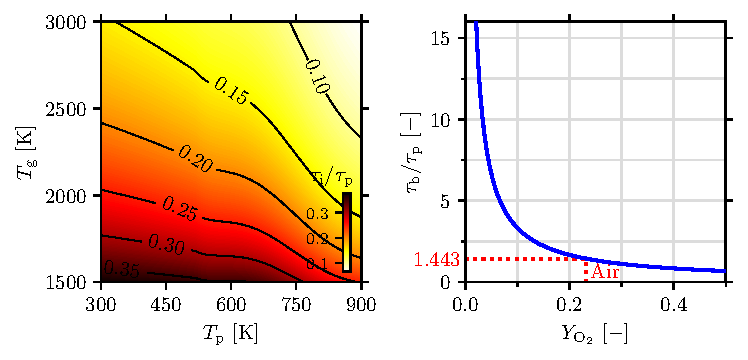
\includegraphics[width=0.9\linewidth]{plots/titbtp.pdf}
    % \vspace{-30pt}
    \caption{Left figure shows the estimation of $\taui/\taup$ at various $T_\mrm{p}$ vs. $T_\mrm{g}$; Right figure shows the estimation of $\taub/\taup$ with respect to $Y_\mrm{O_2}$.}
    \label{fig:titp}
\end{figure}

\subsection{Comparison between combustion timescale $\tau_\mathrm{b}$ and particle relaxation timescale $\tau_\mathrm{p}$}

Equations \ref{eq:taup}, \ref{eq:taub} give $\taub/\taup$ as:
\begin{equation}
    \frac{\taub}{\taup} = \frac{3 \mrm{Sc}_\mrm{O_2}}{2 s_\mrm{FeO}Y_\mrm{O_2}} \label{eq:taubp}
\end{equation}

\noindent where $\mrm{Sc}_\mrm{O_2} = \nu_\mrm{g}/D_\mrm{O_2}$ is the Schmidt number of $\mrm{O_2}$ -- the ratio of viscous and mass diffusivities of oxygen. In the considered ranges of $T_\mrm{g}$ and $Y_\mrm{O_2}$, $\mrm{Sc}_\mrm{O_2} = 0.78 \pm 0.01$ and therefore is assumed constant. Hence, $\taub/\taup$ depends only on $Y_\mrm{O_2}$. For air at $Y_\mrm{O_2} = 0.2323$, $\taub/\taup \approx 1.443$. However, the inverse linear relationship of $\taub/\taup$ with $Y_\mrm{O_2}$ entails $\taub/\taup \rightarrow \infty$ when $Y_\mrm{O_2} \rightarrow 0$. The variation in $\taub/\taup$ with $Y_\mrm{O_2}$ is presented in the right subfigure of Figure \ref{fig:titp} and it is seen that $\taub/\taup$ varies across orders of magnitudes, considerably so at lower $Y_\mrm{O_2}$.\iffalse Note that $Y_\mrm{O_2}$ greater than $0.2323$ (of air) is also considered to examine the sensitivity of the analysis.\fi

% \begin{figure}
%     \centering
%     \begin{subfigure}[b]{0.495\textwidth}
%          \centering
%          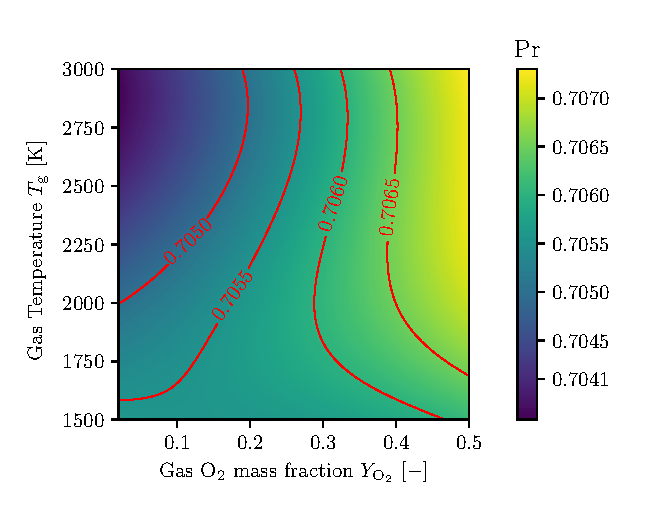
\includegraphics[width=\textwidth]{images/pr.eps}
%          \caption{$\mrm{Pr}$ vs. $T_\mrm{g}$, $Y_\mrm{O_2}$}
%          \label{fig:titpa}
%      \end{subfigure}
%      \hfill
%      \begin{subfigure}[b]{0.495\textwidth}
%          \centering
%          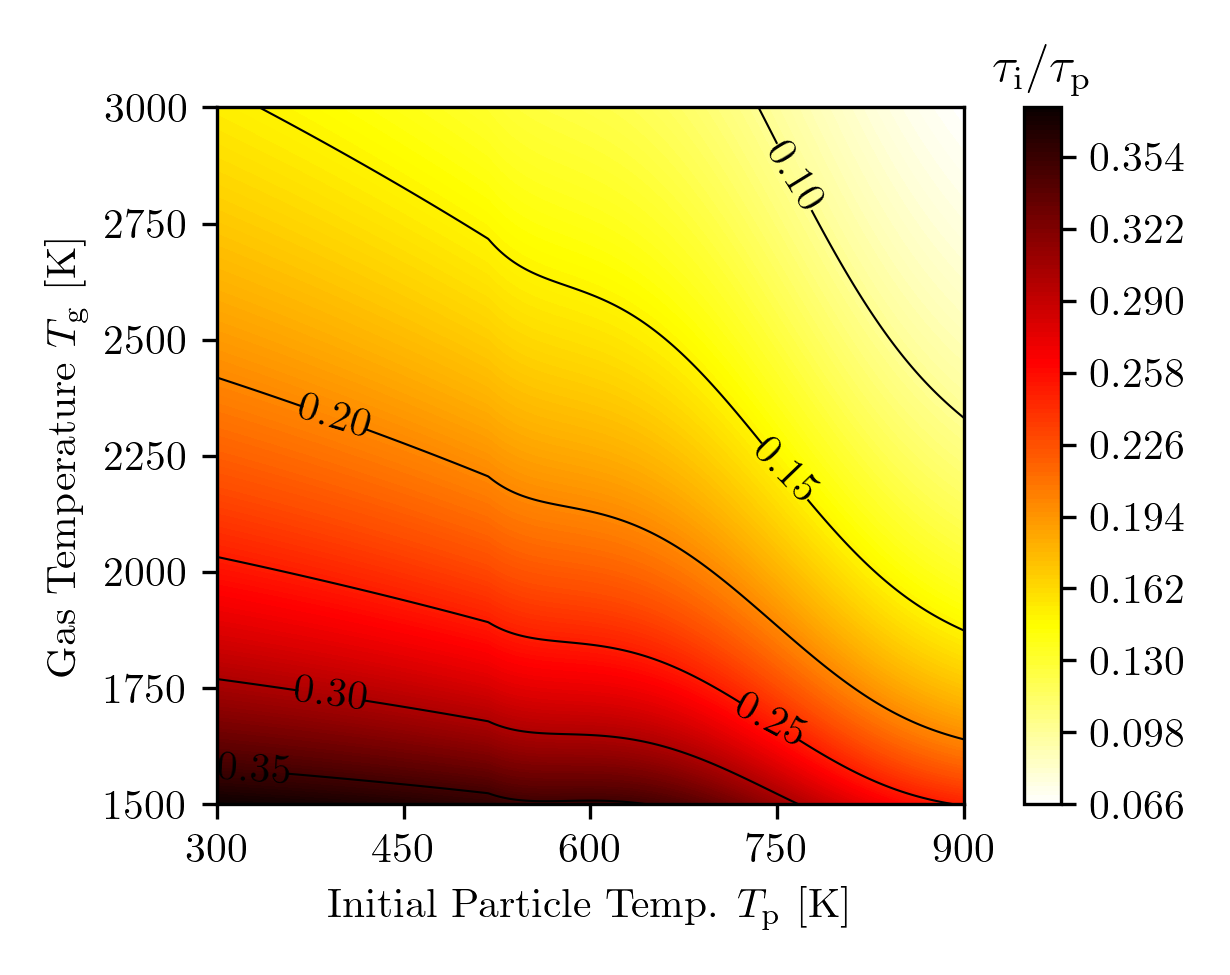
\includegraphics[width=\textwidth]{images/titp.eps}
%          \caption{$\taui/\taup$ vs. $T_\mrm{g}$, $T_\mrm{p}$}
%          \label{fig:titpb}
%      \end{subfigure}
%     \caption{Caption}
%     \label{fig:titp}
% \end{figure}

\iffalse
\begin{figure}[h]
    \centering
    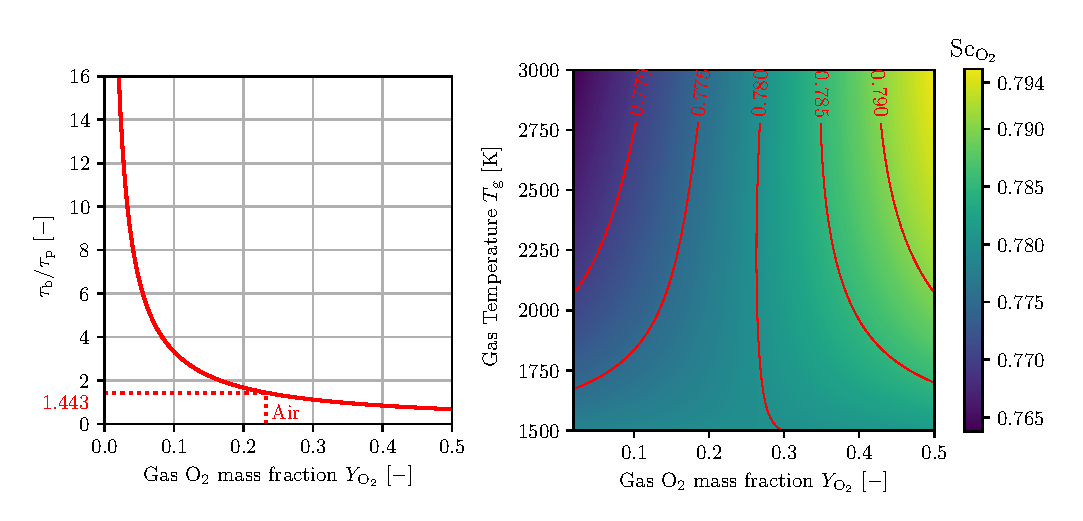
\includegraphics[width=0.95\linewidth]{images/tbtp_2.eps}
    \caption{Left figure shows the estimation of $\taub/\taup$ at various $Y_\mrm{O_2}$; Right figure shows the variation (or lack of) in $\mrm{Sc}$ with $T_\mrm{g}$ and $Y_\mrm{O_2}$.}
    \label{fig:tbtp}
\end{figure}
\fi

\subsection{Comparisons between particle relaxation timescale $\tau_\mathrm{p}$ and cluster formation $\tau_\mathrm{c}$ and evolution $\tau_\mathrm{e}$ timescales }

From Equations \ref{eq:tauc} and the Stokes relation:
\begin{equation}
    \frac{\tauc}{\taup} = 8 \mrm{St}_\eta^{-1} + 5 \label{eq:taucp}
\end{equation}

And from the assumption that $\taue \sim \tauL$:
\begin{equation}
    \frac{\taue}{\taup} = \mrm{Re}_{L}^{1/2}\mrm{St}_\eta^{-1} \label{eq:tauep}
\end{equation}

The variation in $\tauc/\taup$ and $\taue/\taup$ with respect to $\mrm{St}_\eta$ and $\mrm{Re}_L$ is presented in Figure \ref{fig:tauce}. Assuming $\mrm{St}_\eta=1$ and $\mrm{Re}_L > 1000$, $\tauc/\taup = 13$ and $\taue/\taup > 30$. Hence, under these assumptions, $\taui < \taub < \tauc < \taue$, and combustion is likely faster than the time taken for clusters to stabilize and evolve. Note that $\taui$ does not vary across orders of magnitude, and hence preheating can be assumed to be slower than the other processes in typical parameter ranges.

\begin{figure}[h]
    \centering
    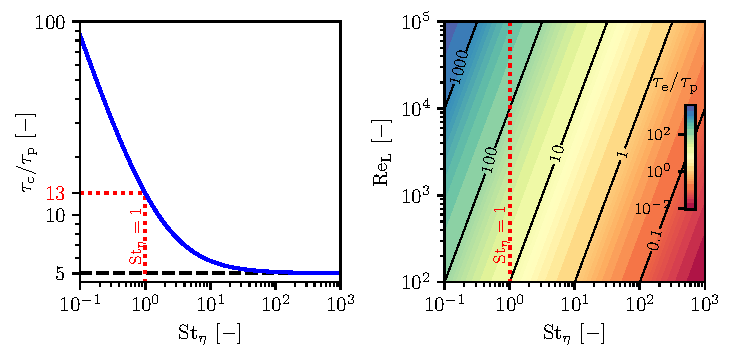
\includegraphics[width=0.9\linewidth]{plots/tctetp2.pdf}
    % \vspace{-30pt}
    \caption{Left figure shows the variation in $\tauc/\taup$ vs. Stokes number $\mrm{St}_\eta$. At $\mrm{St}_\eta=1$, the Equation \ref{eq:taucp} gives $\tauc/\taup = 13$ (indicated by the red dotted line); Right figure shows the variation in $\taue/\taup$ with the bulk Reynolds number $\mrm{Re}_L$ and the Stokes number $\mrm{St}_\eta$. }
    \label{fig:tauce}
\end{figure}

% \section{Discussion on the coupling of cluster formation and evolution with preheating and combustion processes}\label{sec:discussion}

\iffalse The construction of timescale ratios with $\taup$ as reference, as in Equations \ref{eq:tauip}, \ref{eq:taubp}, \ref{eq:taucp}, \ref{eq:tauep}, enables comparison of combustion and clustering timescales with few independent parameters. In the range of $T_\mrm{p}$ and $T_\mrm{g}$ relevant to iron powder combustors, $\taui/\taup < 1$ as evident in Figure \ref{fig:titp}. Assuming $Y_\mrm{O_2} = 0.23$, $\taub/\taup \approx 1.4$. \fi 

\subsection{Comparisons between combustion timescale $\tau_\mathrm{b}$ and cluster formation $\tau_\mathrm{c}$ and evolution $\tau_\mathrm{e}$ timescales }

A comparison of $\taub$ and $\tauc$ can be made by deriving $\taub/\tauc$ from Equations \ref{eq:taubp} and \ref{eq:taucp} as:
\begin{equation}
    \frac{\taub}{\tauc} = \frac{3 \mrm{Sc}_\mrm{O_2}}{2 s_\mrm{FeO}Y_\mrm{O_2} \cdot \left (8\mrm{St}_\eta^{-1} + 5\right)} \label{eq:taubc} 
\end{equation}

Similarly, $\taub/\taue$ is derived from Equations \ref{eq:taubp} and \ref{eq:tauep} as:
\begin{equation}
    \frac{\taub}{\taue} = \frac{3 \mrm{Sc}_\mrm{O_2}}{2 s_\mrm{FeO}Y_\mrm{O_2} \mrm{Re}_L^{1/2}\mrm{St}_\eta^{-1} } \label{eq:taube}
\end{equation}

\begin{figure}
    \centering
    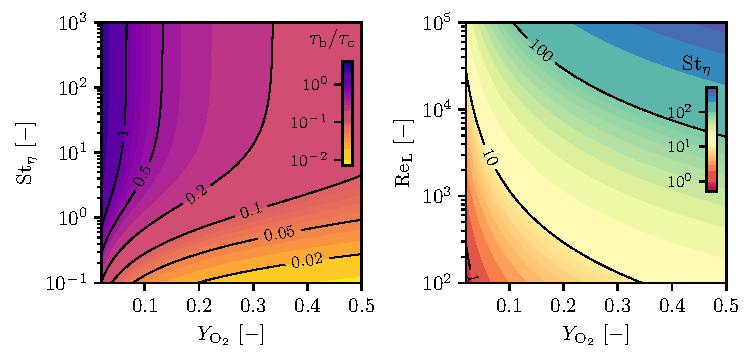
\includegraphics[width=0.9\linewidth]{plots/tctetb3.pdf}
    % \vspace{-30pt}
    \caption{The left figure shows the variation in $\taub/\tauc$ with $Y_\mrm{O_2}$ and $\mrm{St}_\eta$ based on Equation \ref{eq:taubc}. The right figure shows the Stokes number $\mathrm{St}_\eta$ with respect to $Y_\mrm{O_2}$ and $\mrm{Re}_L$ at which $\taub/\taue = 1$, based on Equation \ref{eq:taube}. }
    \label{fig:tctetb}
\end{figure}

These relations, presented in Figure \ref{fig:tctetb}, compares the combustion process with the clustering processes. From the left subfigure it can be seen that under air-like conditions of $Y_\mrm{O_2}$, $\taub < \tauc$ but at lower $Y_\mrm{O_2}$ environments, $\taub \gtrsim \tauc$. Furthermore, the effect of $\mrm{St}_\eta$ on $\taub/\tauc$ decreases when $\mrm{St}_\eta\gg1$, and $\taub/\tauc$ is dependent only on $Y_\mrm{O_2}$ when $\mrm{St}_\eta\gg 1$. The right subfigure of Figure \ref{fig:tctetb} presents $\mrm{St}_\eta$ at which $\taub/\taue = 1$, with $\mrm{Re}_L$ and $Y_\mrm{O_2}$ as axes. Under air-like conditions and typical flow $\mrm{Re}_L \approx 10^4$, $\taub/\taue = 1$ at $\mrm{St}_\eta\approx 60$. Conversely, for the assumed $Y_\mrm{O_2}$ and $\mrm{Re}_L$, $\taub/\taue \approx 1/60$ when $\mrm{St}_\eta \approx 1$. \iffalse Hence, under operating conditions close to air, % $\taub < \tauc$, thus the combustion timescale of the particles is estimated to be less than the time taken for the clusters to fully stabilize. These visualisations, however, do not take into account any predeveloped particle clustering.  the ignited particles would likely complete their co

These relations are presented in Figure \ref{fig:tctetb}, assuming $\mrm{St}=1$. It can be seen from the left figure of Figure \ref{fig:tctetb}, under normal operating conditions of large-scale combustors assuming $\mrm{St}=1$, $\taub<\tauc$, but may approach equivalence when $Y_\mrm{O_2}$ decreases. Hence, the ignited particles would likely complete their combustion process during the time taken for the clusters to stabilize. At lower $Y_\mrm{O_2}$, as $\taub/\tauc$ approaches unity, the dynamics of cluster formation through preferential concentration could interact with the combustion process, and this coupling must be taken into account when considering the design of such combustors. In conditions where the particles are already partially clustered before injection into the combustor, the cluster formation timescale could be lower, and a considerable interaction between the cluster formation dynamics and the combustion process could be expected. \fi

 \iffalse This methodology can be followed to isolate the parameters into coupling regimes based on the value of $\taub/\taue$ at a given $\mrm{Re}_L$, $Y_\mrm{O_2}$ and $\mrm{St}$ such that: when $\taub \ll \taue$, the combustion process in unaffected by the cluster evolution dynamics and the turbulence appears to be ``frozen"; when $\taub \approx \taue$, the combustion process occurs at the same timescale as cluster dynamics and considerable interaction can be expected; when $\taub \gg \taue$, the combustion process is slower than the cluster dynamics that the effect of clustering on combustion is hypothesized to be negligible.
% \iffalse
However, from the right figure of Figure \ref{fig:tctetb}, at $\mrm{Re}_L > 1000$, $\taub \ll \taue$ under realistic $Y_\mrm{O_2}$ conditions. Hence, the cluster evolution dynamics are not expected to interfere with the combustion process and the particle distribution would be ``frozen" from the perspective of particle combustion. Even if the injected particle distribution is partially concentrated, since $\taue \gg \taub$, the particle distribution through the combustion process can be approximated to be static. Hence, the coupling of the cluster evolution dynamics and the combustion process can be neglected.


From Figure \ref{fig:tctetb}, it can be seen that $\taub > \tauc$ when $Y_\mrm{O_2}<0.027$. Hence, under this condition, the combustion process is significantly extended, longer than the cluster formation. In such circumstances, the effects of preferential concentration on the combustion process will be enhanced and noticeable. 

A graphical description of the hypothetical interpretation of $\taub$ with respect to $\tauc$ and $\taue$ is presented in Figure \ref{fig:scenarios}. Depending on $\taub/\tauc$, the coupling between combustion and preferential concentration can be evaluated. If $\taub \ll \tauc$, the effects of preferential concentration on the combustion process can be neglected, since the particles burn out before the particle distribution has stabilized into clusters. If $\taub \gg \taue$, particles freely move out of clusters during their combustion process and hence, the effect of preferential concentration on the combustion would be minimized. The effects of preferential concentration on the combustion process are hence hypothesized to be maximum when $\tauc < \taub < \taue$. This regime can be described as particles undergoing the combustion process which is longer than the stabilization time of cluster formation, yet shorter than the evolution time of the clusters.  A numerical or experimental investigation into the multiple regimes hypothesized in this work will be essential in identifying the dynamic properties that do not fit in this analysis.

\fi

\iffalse
\begin{figure}
    \centering
    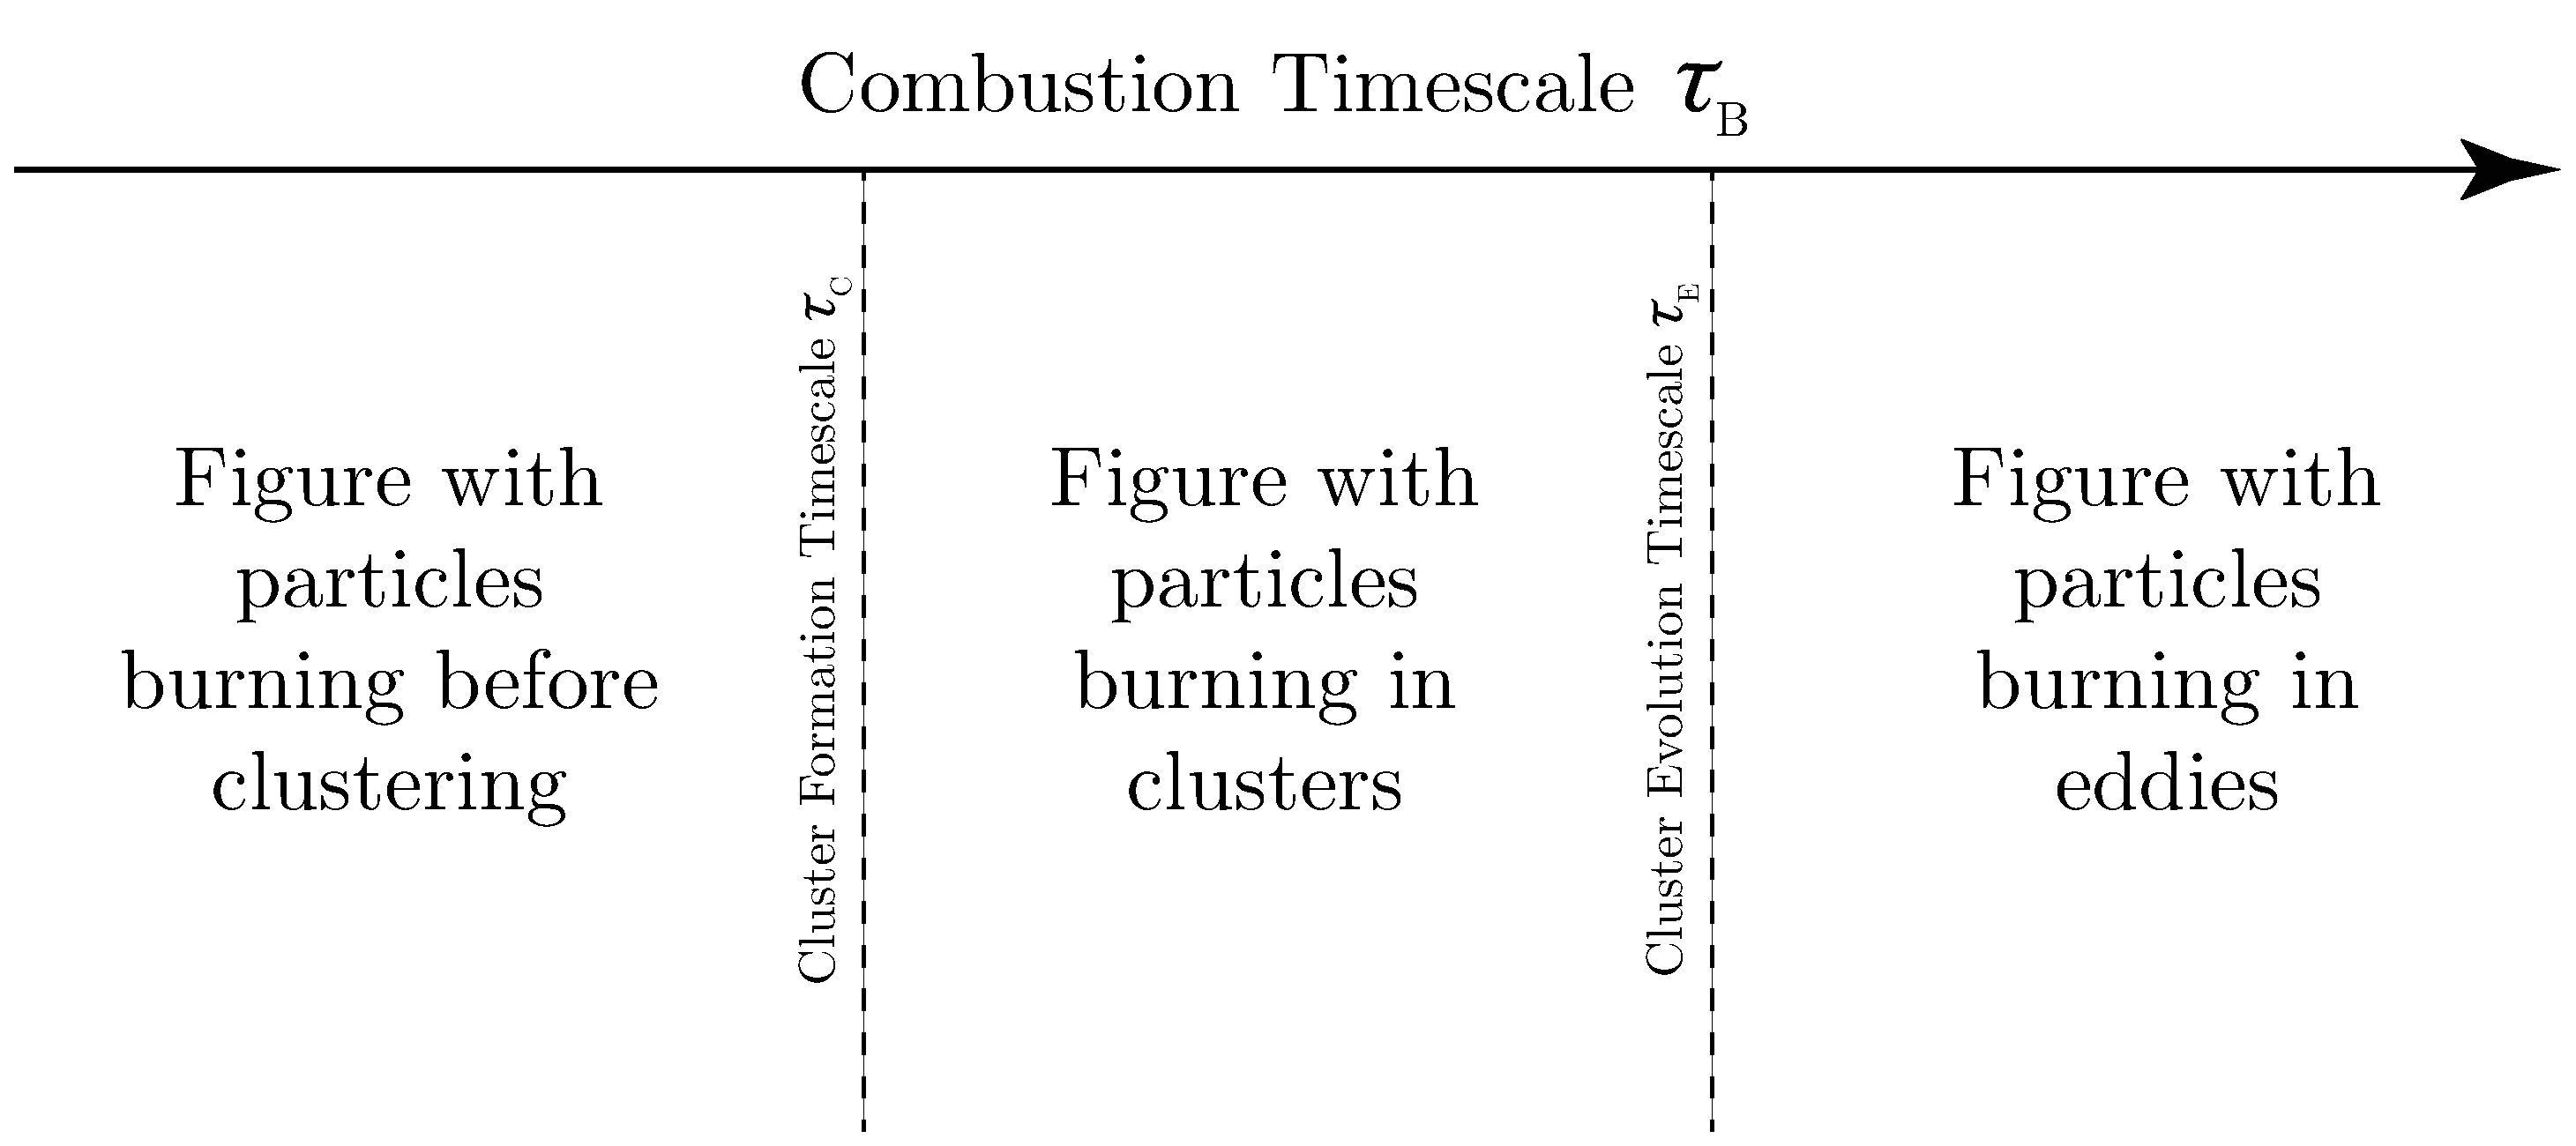
\includegraphics[width=\linewidth]{images/scenarios.eps}
    \caption{A graphical representation of the flow and combustion regimes based on the combustion dynamics represented by $\taub$ in regard to clustering dynamics represented by $\tauc$ and $\taue$.}
    \label{fig:scenarios}
\end{figure}
\fi

\subsection{Interpretation of coupling regimes of combustion and clustering processes}

{\pink This analysis presents the key relationships (Eqs.~\ref{eq:taubc} and \ref{eq:taube}), shown in Figure~\ref{fig:tctetb}, which enable the evaluation of the degree of coupling or decoupling among combustion, turbulence, and clustering processes, based on $Y_\mrm{O_2}$, $\mrm{St}_\eta$, and $\mrm{Re}_L$ as follows:
\begin{dingautolist}{192}
\setlength\itemsep{0em}
    \item If $\taub/\tauc \ll 1$, the combustion processes are completed before the formation of clusters, and hence, the process of clustering through preferential concentration can be, for the most part, neglected. However, in this case, the initial particle distribution becomes relevant. 
    \item If $\taub/\tauc \gtrsim 1$ and $\taub/\taue \ll 1$, the cluster formation process is relevant in the combustion process, as the particles are expected to stabilize into clusters during or before the combustion is complete. Most particles are likely to combust completely in clusters, as the cluster evolution is longer than the combustion timescale, and hence transport out of clusters is weak. In this case, the effects of particle clustering through preferential concentration are maximized.
    \item If $\taub/\taue \gtrsim 1$, the particles cluster, but also move around the domain across multiple clusters during combustion. This ensures the availability of oxygen through their combustion process, and the effect of particle clustering is minimized.
\end{dingautolist}

With this analysis, it can be inferred that in the regimes \Pisymbol{pzd}{192} and \Pisymbol{pzd}{194}, combustion and preferential concentration are effectively uncoupled, and clustering can be neglected. 

\section{Summary of key findings}\label{sec:conclusion}

In summary, the particle timescales of relaxation $\taup$, preheating $\taui$ and combustion $\taub$ are derived based on assumptions motivated by recent research. The timescales of preferential concentration -- cluster formation $\tauc$ and cluster evolution $\taue$ are estimated from research into the phenomena, assuming that the particles are distributed as a Poisson distribution in a flow with homogeneous isotropic turbulence. Comparison of the timescales indicates: $\taui$ is much smaller than the other timescales for temperature ranges relevant to larger combustors; $\taub/\taup$ depends only on the gas oxygen mass fraction $Y_\mrm{O_2}$; estimating $\taub/\tauc$ and $\taub/\taue$ based on the Stokes number $\mrm{St}_\eta$, integral scale Reynolds number $\mrm{Re}_L$ and $Y_\mrm{O_2}$ can be helpful in identifying ranges where the combustion and clustering are uncoupled.} {\blue This analysis is not more than an idealized thought experiment. Several assumptions made do not coincide directly with realistic scenarios -- scenarios that have several complex dynamic phenomena that cannot be feasibly incorporated in this analysis. Therefore, instead of precisely describing any real-world iron-powder combustor, this analysis and the discussion presented aim to act as a guide for further extensive research in identifying (and eliminating) where preferential concentration would have a minimal or negligible effect on the combustion process.}

\iffalse
Hence, this analysis is not meant to be interpreted \textit{directly} to real-world applications. Rather, this analysis and the discussion presented aim to act as \textit{a guideline for further extensive research in identifying (and eliminating) where preferential concentration would have minimal or negligible effect on the combustion process}. Further detailed research incorporating all of the necessary dynamic processes is still essential in the complete understanding of the coupling of the phenomena.
\fi
\iffalse
A simplified theoretical analysis of the combustion and the particle clustering timescales is presented. The particle timescales -- relaxation $\taup$, preheating $\taui$ and combustion $\taub$ -- can be expressed as dependent on the particle size as $d_\mrm{p}^2$. Consequently, $\taui/\taup$ and $\taub/\taup$ are independent of particle size, and exhibit few dependent parameters. The flow timescales -- Kolmogorov timescale $\tauk$ and integral timescale $\tauL$ -- can be described through the Stokes number $\mrm{St}$ and the Reynolds number $\mrm{Re}_{L}$. The clustering timescales -- cluster formation timescale $\tauc$ and cluster evolution timescale $\taue$ -- can be expressed as a function of the flow timescales. This construction enables a simplified comparison of the phenomena using few independent parameters. In conditions resembling large scale iron powder combustors, $\taui$ is smaller than $\taub$ and hence, the preheating timescale can be neglected as negligibly small in most cases. The generalized comparison of $\taub$ with $\tauc$ and $\taue$ is derived, and in air-like conditions, $\taub < \tauc$, but could be in the same order of magnitude at lower $Y_\mrm{O_2}$. An analysis on $\taub/\taue$ depending on $\mrm{St}$, $\mrm{Re}_L$ and $Y_\mrm{O_2}$ yields a regime map based on which the interaction between the combustion process and the cluster dynamics can be predicted.  Thus, the cluster formation dynamics are expected to interact with the combustion process.  However, $\taub \ll \taue$ at $\mrm{Re}_L>1000$, and hence, the cluster evolution dynamics are not expected to interact with the combustion process, and can be neglected. \fi

\bibliographystyle{elsarticle-num} 
\bibliography{references}

\end{document}

\endinput
%%
%% End of file `elsarticle-template-num.tex'.
